\section{مدل علّی}
پیدا کردن تعریفی برای علت واقعی%
\lf{Actual Cause}
مبحثی است که مورد مطالعه و تحقیق بسیاری قرار گرفته است.
این مساله به طور خاص در متون فلسفه مورد توجه قرار گرفته است.
یکی از تعاریف علت واقعی که مورد توجه بسیاری قراری گرفته است، تعریفی مبتنی بر وابستگی خلاف واقع%
\lf{Counterfactual}
است.
مطابق این تعریف، رویداد الف علت رویداد ب است اگر در شرایطی که رویداد الف اتفاق نیافته باشد، رویداد ب هم اتفاق نیافتند.
در اینجا اتفاق نیفتادن رویداد الف خلاف واقع است، چون در سناریوی واقعی
(سناریو ای که واقعا اتفاق افتاده و مشاهده شده است)
رویداد الف اتفاق افتاده است و در نظر گرفتن شرایطی که در آن رویداد الف اتفاق نیفتاده باشد بر خلاف واقعیت موجود است.
اما این مدل به تنهایی امکان پیدا کردن علت مناسب را در همه‌ی موارد ندارد.
به عنوان مثال سناریوی زیر را در نظر بگیرید که در آن سارا و بهرام هر کدام یک سنگ را برداشته و به سمت یک بطری شیشه‌ای پرتاب می‌کنند.
در این سناریو، سنگ سارا زودتر از سنگ بهرام به بطری برخورد کرده و در نتیجه آن را می‌شکند.
در این سناریو واضح است که پرتاب سنگ توسط سارا علت شکسته شدن بطری است.
فرض کنید بخواهیم از علیت مبتنی بر خلاف واقع برای پیدا کردن این علت استفاده کنیم.
بنابراین باید شرایطی را در نظر بگیریم که سارا سنگ خود را پرتاب نکند.
اما مشکل اینجاست که در این شرایط همچنان بطری شکسته می‌شود، چون اگر سارا سنگ خود را پرتاب نکند، بهرام همچنان سنگ خود را پرتاب می‌کند و در نتیجه این بار سنگ بهرام به بطری برخورد کرده و آن را می‌شکند.
بنابراین در این سناریو امکان تعریف پرتاب سنگ توسط سارا به عنوان علت شکسته شدن بطری با استفاده از استدلال مبتنی بر خلاف واقع وجود ندارد.
هالپرن%
\lf{Halpern}
و پرل%
\lf{Pearl}
برای حل کردن مشکلاتی از این دست، تعریف جدیدی از علت واقعی
\cite{hp}
ارائه کردند.
مدل ارائه شده توسط آن‌ها به دلیل اینکه مبنای ریاضی دارد امکان استفاده از آن را در آنالیز و تحلیل سیستم‌های محاسباتی فراهم می‌کند.
به همین دلیل این تعریف در مقالات زیادی در حوزه‌ی دانش کامپیوتر مورد استفاده قرار گرفته است.
برای تعریف علت واقعی ابتدا برخی مفاهیم اولیه مورد استفاده در این تعریف توضیح داده می‌شوند.
به صورت کلی فرض می‌شود که دنیای مورد تحلیل توسط تعدادی متغیر تصادفی مدل شده است.
اگر
$X$
یک متغیر تصادفی باشد، یک رویداد به شکل
$X=x$
تعریف می‌شود.
برخی از این متغیر‌ها بر روی یکدیگر تاثیر گذارند.
این وابستگی‌ها در قالب مجموعه‌ای از معادلات ساختاری%
\lf{Structural Equations}
مدل می‌شوند.
هر یک از این معادلات در واقع یک مکانیزم یا قانون مشخص در این دنیا را مدل می‌کنند.
متغیرها به دو دسته درونی%
\lf{Endogenous}
و برونی%
\lf{Exogenous}
تقسیم می‌شوند.
متغیر‌های برونی متغیر‌هایی در نظر گرفته می‌شوند که مقدار آن‌ها توسط عواملی که درون مدل نیستند تعیین می‌شوند.
بنابراین در یک مدل علی فرض می‌شود که مقدار این متغیر‌ها از قبل مشخص است.
اما متغیر‌های درونی متغیرهایی هستند که مقدار آن‌ها بر اساس معادلات ساختاری تعیین می‌شود.
به صورت دقیق‌تر، امضای%
\lf{Signature}
یک مدل یک سه‌تایی
$\mc{S} = (\mc{U},\mc{V},\mc{R})$
است که در آن
$\mc{U}$
مجموعه‌ی متغیر‌های بیرونی
$\mc{V}$
مجموعه‌ی متغیر‌های درونی و
$\mc{R}$
دامنه‌ی مقادیر ممکن برای هر یک از متغیر‌ها را مشخص می‌کند.
در این مدل فرض می‌شود که مجموعه‌ی متغیر‌های درونی محدود است.
مدل علّی بر روی یک امضای
$\mc{S}$
یک دوتایی
$\mc{M} = (\mc{S},\mc{F})$
است که در آن
$\mc{F}$
به هر متغیر داخلی
$X \in \mc{V}$
یک تابع
$F_X: \times_{Z\in ((\mc{U}\cup \mc{V})\setminus \s{X})}R(Z)
\rightarrow \mathcal{R}(X)$
اختصاص می‌دهد.
نشانه‌گذاری
$\times_{Z\in ((\mc{U}\cup \mc{V})\setminus \s{X})}$
ضرب خارجی%
\lf{Cross-Product}
مجموعه‌های
$\mc{R}(Z)$
را به ازای تمام متغیر‌هایی مانند 
$Z$
در 
$(\mc(U)\cup \mc{V}) \setminus \s{X}$
مشخص می کند.
بنابراین اگر فرض کنیم
$(\mc{U}\cup \mc{V})\setminus \s{X} = \s{Z_1,...,Z_k}$
، آنگاه 
$\times_{Z\in ((\mc{U}\cup \mc{V})\setminus \s{X})}\mc{R}(Z)$
متشکل از چندتایی‌هایی به شکل
$(z_1,...,z_k)$
است که به ازای 
$i = 1,...,k$
هر 
$z_i$
یک مقدار ممکن برای متغیر 
$Z_i$
است.
هر تابع، معادله‌ی یک متغیر را به ازای مقادیر تمام متغیر‌های دیگر مشخص می‌کند.
به عنوان مثال اگر فرض کنیم
$F_X(Y,Z,U) = Y + U$
اگر داشته باشیم
$Y=3, U=2$
آنگاه مقدار
$X$
برابر ۵ خواهد شد.
این معادلات امکان تفسیر آن‌ها بر اساس شرایط خلاف واقع را می‌دهند.
به عنوان مثال در همین مدل اگر فرض کنیم که
$U=u$
می‌توانیم نتیجه بگیریم که اگر مقدار متغیر
$Y$
برابر ۴ باشد آنگاه مستقل از اینکه مقدار بقیه‌ی متغیر‌ها در دنیای واقعی چه مقداری دارند، مقدار متغیر
$X$
برابر
$u+4$
خواهد بود که به صورت
$(M,u) \vDash [Y \la 4](X = u + 4)$
نوشته می‌شود.
توابع ذکر شده فقط برای متغیر‌های درونی تعریف می‌شوند و همانطور که پیش‌تر اشاره شد، برای متغیرهای بیرونی تابعی تعریف نمی‌شود و فرض می‌شود که مقدار آن‌ها از قبل مشخص شده است
\cite{Halpern_2016}.

\begin{example}
      \label{ex:hp:fire}
      یک جنگل را در نظر بگیرید که می‌تواند توسط رعد و برق یا یک کبریت رها شده دچار آتش سوزی شود.
      برای مدل کردن این سناریو از سه متغیر بولی%
      \lf{Boolean}
      استفاده می‌کنیم:
      \begin{itemize}
            \item متغیر
                  $F$
                  که اگر جنگل دچار آتش سوزی شود مقدار آن درست است و در غیر این صورت مقدار آن غلط است
            \item متغیر
                  $L$
                  که اگر رعد و برق اتفاق افتاده باشد مقدار آن درست است و در غیر این صورت غلط است
            \item متغیر
                  $M$
                  که اگر یک کبریت در جنگل رها شده باشد مقدار آن درست است و در غیر این صورت غلط است
      \end{itemize}
\end{example}
در این مثال فرض می کنیم که مقادیر متغیر‌های برونی به گونه‌ای است که تمام شرایط لازم برای آتش سوزی جنگل در صورتی که رعد و برق اتفاق بیافتد یا کبریتی در جنگل رها شود را دارد
(به عنوان مثال درختان جنگل به اندازه‌ی کافی خشک هستند و اکسیژن کافی در هوا وجود دارد).
در این مدل تابع متغیر
$F$
را به گونه‌ای تعریف می‌کنیم که داشته باشیم:
$F_F(\vec u, L , M) = L \vee M$.
همانطور که پیش‌تر بیان شد، این مدل علّی امکان بررسی معادلات بر اساس شرایط خلاف واقع را می‌دهد.
به صورت دقیق‌تر اگر
$M = (\mc{S},\mc{F})$
یک مدل علی،
$\vec X$
یک بردار از متغیرهای درونی و
$\vec{x}, \vec{u}$
برداری از مقادیر متغیر‌های
$\vec{X},\mc{U}$
باشند
مدل
$M_{\vec{X}\la \vec{x}}$
را با امضای
$S_{\vec X}=(\mc{U},\mc{V}-\vec X,\mc{R}|_{\mc{V} \setminus \vec{X}})$
یک زیرمدل%
\lf{Sub-Model}
از
$M$
تعریف می‌کنیم که در آن
$\mc{R}|_{\mc{V}\setminus \vec X}$
محدود کردن 
$\mc{R}$
به متغیر‌های داخل 
$\mc{V} \setminus \vec X$
است.
به صورت شهودی این مدل حاصل مداخله‌%
\lf{Intervention}
ای در مدل
$M$
است که در آن مقادیر
$\vec{x}$
را به متغیر‌های
$\vec{X}$
اختصاص داده‌ایم.
به صورت دقیق‌تر تعریف می‌کنیم
$M_{\vec{X}\la\vec{x}} = (\mc{S}_{\vec{X}},\mc{F}^{\vec{X}\la\vec{x}})$
که
$F_Y^{\vec{X}\la\vec{x}}$
از تابع
$F_Y$
که در آن مقادیر
$\vec{x}$
را به متغیرهای
$\vec{X}$
اختصاص داده‌ایم به دست می‌آید.
به عنوان مثال اگر
$M$
مدل مثال
\ref{ex:hp:fire}
باشد آنگاه در مدل
$M_{L\la \F}$
معادله‌ی متغیر
$F$
به
$F = M$
تبدیل می‌شود.
این معادله دیگر به متغیر
$L$
وابسته نیست بلکه با توجه به مقدار آن که در اینجا غلط است معادله‌ی جدیدی دارد.
علاوه براین توجه کنید که در مدل
$M_{L\la \F}$
دیگر معادله‌ای برای متغیر
$L$
وجود ندارد.
توجه کنید که در حالت کلی ممکن است یک بردار یکتا از مقادیر متغیر‌ها برای یک مدل وجود نداشته باشد که همزمان تمامی معادلات را حل کند.
در مدل علّی یک بردار از مقادیر متغیر‌های برونی
$\vec u$
یک هم‌بافت%
\lf{Context}
نامیده می‌شود.
در مدل‌های بازگشتی به ازای یک هم‌بافت مشخص همیشه یک راه‌حل یکتا برای تمامی معادلات مدل وجود دارد.
در ادامه فرض می‌شود که مدل‌ها بازگشتی هستند. تعمیم مدل‌ علّی برای مدل‌های غیربازگشتی در
\cite{hp}
توضیح داده است.
برای یک مدل می‌توان یک شبکه‌ی علّی ترسیم کرد.
این شبکه یک گراف جهت‌دار است که به ازای هر متغیر یک گره در آن وجود دارد و یک یال بین دو گره وجود دارد اگر تابع متغیر دوم به متغیر اول وابسته باشد.
به عنوان مثال شکل زیر شبکه‌ی علّی مثال
\ref{ex:hp:fire}
را نشان می‌دهد:
\begin{center}
      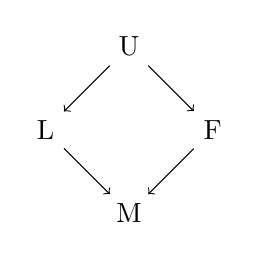
\begin{tikzpicture}[node distance={15mm}]
            \node (l) {L};
            \node (m) [below right of=l]  {M};
            \node (f) [above right of=m] {F};
            \node (u) [above right of=l] {U};
            \draw [->] (l) -- (m);
            \draw [->] (f) -- (m);
            \draw [->] (u) -- (l);
            \draw [->] (u) -- (f);
      \end{tikzpicture}
\end{center}
در ادامه برای سادگی رسم شبکه‌ی علی، متغیر‌های برونی را از آن‌ها حذف می‌کنیم.
\subsection{علت واقعی}
در ادامه‌ فرمول‌های لازم برای تعریف علت واقعی توصیف می‌شوند.
اگر
$\mc{S} = (\mc{U},\mc{V},\mc{R})$
یک امضا باشد فرمول
‍‍$X=x$
یک رویداد بدوی%
\lf{Prime Event}
نامیده می‌شود که
‍$X \in \mc{V},x \in \mc{R}(X)$.
فرمول
$[Y_1 \la y_1,...,Y_k\la y_k]\varphi$
یک فرمول علّی پایه%
\lf{Basic Causal Formula}
نامیده می‌شود که در آن:
\begin{itemize}
      \item $\varphi$
            یک ترکیب بولی از رویداد‌های بدوی است
      \item $Y_1,...,Y_k$
            متغیر‌های متمایز در
            $\mc{V}$
            هستند
      \item $y_i \in \mc{R}(Y_i)$
\end{itemize}
این فرمول به صورت خلاصه به شکل
$[\vec{Y}\la \vec{y}]\varphi$
نوشته می‌شود و اگر
$k=0$
باشد آنگاه به صورت
$\varphi$
نوشته می‌شود.
به صورت شهودی یک فرمول به شکل
$[\vec{Y}\la \vec{y}]\varphi$
بیان می‌کند که در شرایط خلاف واقع‌ ای که در آن مقادیر
$\vec{y}$
به متغیر‌های
$\vec{Y}$
اختصاص داده شده است فرمول
$\varphi$
برقرار است.
یک فرمول علّی به صورت یک ترکیب بولی از فرمول‌های علّی پایه تعریف می‌شود.
برقراری فرمول علی
$\psi$
در مدل
$M$
تحت هم‌بافت
$\vec u$
را به صورت
$(M,\vec u) \vDash \psi$
نشان می‌دهیم.
به عنوان مثال
$(M,\vec{u}) \vDash [\vec{Y}\la \vec{y}](X=x)$
برقرار است اگر مقدار متغیر
$X$
در راه حل معادلات مدل
$M_{\vec{Y}\la \vec{y}}$
تحت هم‌بافت
$\vec u$
برابر
$x$
باشد.

\begin{definition}
      \label{def:cause}
      فرمول
      $\vec X = \vec x$
      علت واقعی
      $\varphi$
      (
      که تاثیر%
      \lf{Effect}
      نامیده می‌شود)
      در
      $(M,\vec{u})$
      است
      اگر شرایط زیر برای آن برقرار باشد:
      \begin{enumerate}
            \item $(M,\vec{u}) \vDash (\vec{X} = \vec{x}) \wedge \varphi$
            \item یک افراز مانند
                  $(\vec{Z},\vec{W})$
                  از مجموعه‌ی متغیر‌های
                  $\mc{V}$
                  با شرط
                  $\vec{X} \subseteq \vec{Z}$
                  و مقادیر
                  $(\vec{x},\vec{w}')$
                  برای متغیر‌های
                  $(\vec{X},\vec{W})$
                  وجود داشته باشد که داشته باشیم
                  $(M,\vec{u})\vDash \vec{Z} = \vec{z}^*$
                  و شرایط زیر را برآورده کند:
                  \begin{enumerate}
                        \item $(M,\vec u)\vDash[\vec{X}\la\vec{x}',\vec{W}\la\vec{w}']
                                    \neg \varphi$
                        \item $\forall \vec{W'} \subseteq \vec{W},\vec{Z'}\in \vec{Z}.
                                    (M,\vec{u})\vDash [\vec X\la\vec x,\vec{W}'\la \vec{w}',\vec{Z}'\la \vec{z}^*]\varphi$
                  \end{enumerate}
            \item $\vec X$
                  مینیمال باشد.
      \end{enumerate}
\end{definition}
در این تعریف شرط اول بیان می‌کند که علت و تاثیر هر دو در شرایط واقعی برقرار هستند.
شرط دوم به دنبال پیدا کردن شرایطی است که تحت آن تاثیر به صورت غیر واقع به علت وابسته باشد.
این شرایط متغیرهای
$\vec W$
و مقادیری مانند
$\vec{w}'$
برای آن‌ها هستند.
شرط ۲.آ بررسی می‌کند که تحت شرایطی که توسط
$\vec W \la \vec{w}'$
به وجود می‌آید اگر علت مقداری متفاوت از مقدار خود در هم‌بافت واقعی داشته باشد اثر در مدل دیده نمی‌شود.
شرط ۲.ب بررسی می‌کند که شرایط
استفاده شده در ۲.آ عامل
از بین رفتن اثر در ۲.آ نباشند.
برای این منظور در شرایطی که علت مقدار واقعی خود را دارد در تمامی حالت‌هایی که متغیر‌های شرایط می‌توانند داشته باشند بررسی می‌شود که اثر همچنان برقرار باشد.
شرط سوم در واقع بیان می‌کند که زیرمجموعه‌ای از علت وجود نداشته باشد که همزمان شرایط ۱ و ۲ را برقرار کند.
در تعریف بالا
$(\vec W, \vec w',\vec x')$
یک شاهد%
\lf{Witness}
بر اینکه
$\vec X = \vec x$
علت
$\varphi$
است تعریف می‌شود.

\subsection{پیدا کردن علت واقعی در مسائل}

در ادامه مثال سارا و بهرام که در ابتدای این بخش ذکر شده بود را بررسی می‌کنیم.

برای مدل کردن این مساله متغیر‌های زیر را در نظر می‌گیریم:
\begin{itemize}
      \item $BT$:
            پرتاب سنگ توسط بهرام
      \item $BH$
            برخورد سنگ بهرام به بطری
      \item $ST$:
            پرتاب سنگ توسط سارا
      \item $SH$:
            برخورد سنگ سارا به بطری
      \item $BS$:
            شکسته شدن بطری
\end{itemize}

\begin{figure}
      \centering
      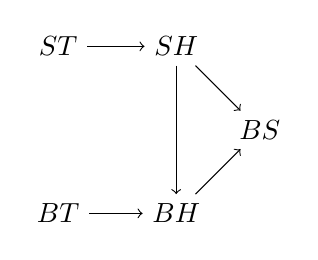
\begin{tikzpicture}[node distance={15mm}]
            \node (bs)  {$BS$};
            \node (sh) [above left of=bs] {$SH$};
            \node (bh) [below left of=bs] {$BH$};
            \node (st) [left of=sh]{$ST$};
            \node (bt) [left of=bh] {$BT$};
            \draw [->] (st) -- (sh);
            \draw [->] (sh) -- (bh);
            \draw [->] (bt) -- (bh);
            \draw [->] (sh) -- (bs);
            \draw [->] (bh) -- (bs);
      \end{tikzpicture}
      \caption{}
      \label{fig:hp:sb}
\end{figure}
ابتدا فرض می‌کنیم که متغیر‌های
$BT,ST$
تنها به متغیر‌های برونی وابسته‌اند.
بطری در صورتی شکسته می‌شود که هر یک از سنگ‌های سارا یا بهرام با آن برخورد کنند.
بنابراین برای شکسته شدن بطری معادله‌ی
$BS = BH \vee SH$
را در نظر می‌گیریم.
نکته‌ی اصلی در این مساله این است که سنگ سارا زودتر از سنگ بهرام به شیشه برخورد می‌کند، به همین دلیل لازم است تا این موضوع در مدل لحاظ شود.
یک راه برای مدل کردن این مساله این است که معادله‌ی برخورد سنگ بهرام به شیشه را به گونه‌ای تعریف کنیم که تنها در صورتی که سنگ سارا به بطری برخورد نکرده باشد آنگاه سنگ بهرام به بطری برخورد کند.
بنابراین می‌توانیم معادله‌ی
$BH = BT \wedge \neg SH$
را تعریف کنیم.
علاوه بر این معادله‌ی برخورد سنگ سارا را بدون وابستگی به برخورد سنگ بهرام تعریف می‌کنیم:
$SH = ST$.
با توجه به این تعاریف برای معادلات می‌توانیم گراف علّی شکل
\ref{fig:hp:sb}
را برای این مدل رسم کنیم
در این مدل می‌توانیم
$ST = \T$
را به عنوان علت
$BS = \T$
تعریف کنیم.
برای برقراری شرط ۲ در تعریف علت واقعی شرایط
$\vec W = \s{BT}$
و
$w' = \F$
را در نظر می‌گیریم.
در این شرایط چون مقدار
$BH$
برابر
$\F$
می‌شود، مقدار
$BS$
تنها وابسته به مقدار
$SH$
و در نتیجه
$ST$
می‌شود.
همچنین در این مدل
$BT = \T$
علت شکسته شدن شیشه نیست.
مثلا فرض کنید که شرایط
$\vec W = \s{ST},w' = \F$
را در نظر بگیریم.
در این شرایط اگر مقدار
$BT$
را به
$\F$
تغیر دهیم مقدار
$BS$
هم غلط می‌شود.
بنابراین شرط ۲.آ برقرار است.
اما به ازای
$\vec Z' = \s{BH}$
شرط ۲.ب برقرار نمی‌شود.
در این حالت داریم:
$(M,\vec{u})\vDash[BT \la \T,ST \la \F,BH \la F]BS = \F$
توجه کنید با وجود اینکه مقدار درست به
$BT$
اختصاص یافته اما چون مقدار
$BH$
به مقدار آن در هم‌بافت واقعی برگردانده می‌شود در نتیجه مقدار
$BS$
همچنان غلط می‌ماند.

مثال بالا نشان می‌دهد که این تعریف از علت واقعی برخی از مشکلات موجود در تعاریف ساده مبتنی بر خلاف واقع را برطرف می‌کند و می‌تواند توضیح مناسبی در برخی از این مثال‌ها پیدا کند.
نکته‌ای که باید به آن توجه شود این است که هنوز روش یا معیاری برای این که چه تعریفی از علت واقعی تعریف مناسب است وجود ندارد.
تنها روش ممکن مقایسه تعاریف مختلف استفاده از آن‌ها در مساله‌ها و سناریوهای مختلف و بررسی تطابق علت به دست آمده با استفاده از این تعریف‌ها با شهود موجود از مساله است.

\subsection{مدل تعمیم‌یافته}
مدل علّی تعمیم یافته%
\lf{Extended Causal Model}
یک سه‌تایی
$(\mc{S},\mc{F},\mc{E})$
است که
$(\mc{S},\mc{F})$
یک مدل علّی است و
$\mc{E}$
یک مجموعه از مقداردهی‌های مجاز%
\lf{Allowable Settings}
برای متغیر‌های درونی است.
به صورت دقیق‌تر اگر متغیر‌های درونی
$X_1,...,X_n$
باشند آن‌گاه
$(x_1,...,x_n) \in \mc{E}$
اگر
$X_1=x_1,...,X_n=x_n$
یک مقداردهی مجاز است.
یک مقداردهی دلخواه به یک زیرمجموعه از متغیر‌های درونی مجاز است اگر امکان تعمیم به یک مقداردهی مجاز در
$\mc{E}$
را داشته باشد.
هدف از این تعریف جلوگیری از در نظر گرفتن علت‌هایی است که شرایط رخ دادن آن‌ها غیر محتمل است.
با توجه به تعریف مقداردهی مجاز، علت واقعی در یک مدل تعمیم یافته به گونه‌ای تعریف می‌شود که در شرط ۲ فقط امکان مقداردهی‌های مجاز وجود داشته باشد.
در
\cite{hp}
تعریف دقیق علت واقعی در مدل تعمیم یافته بیان نشده است.
در بخش بعدی تعریفی از علت واقعی در مدل تعمیم یافته ارائه می‌شود.

\subsection{علت واقعی بدون شرط}
فرض کنید که
$\vec X = \vec x$
یک علت واقعی برای
$\varphi$
در
$(M,\vec u)$
با استفاده از شاهد
$(\e,\e,\vec x')$
باشد.
با توجه به اینکه در اینجا
$\vec W$
یک بردار خالی است پس عملا شرط ۲.ب به بررسی شرط زیر تبدیل می‌شود:
\begin{align*}
      \forall \vec{Z'}\in \vec{Z}.
      (M,\vec{u})\vDash [\vec X\la\vec x,\vec{Z}'\la \vec{z}^*]\varphi
\end{align*}
با دقت در شرط بالا می‌توان دریافت که مقدار متغیر‌ها در فرمول‌های
$[\vec X\la\vec x,\vec{Z}'\la \vec{z}^*]\varphi $
با مقدار متغیر‌ها در هم‌بافت اولیه تفاوتی ندارد زیرا مقدار آن‌ها به مقداری که در هم‌بافت اولیه داشته‌اند برگردانده می‌شود.
بنابراین در شرط بالا می‌توان نتیجه گرفت:
\begin{align*}
      (M,\vec{u})\vDash [\vec X\la\vec x,\vec{Z}'\la \vec{z}^*]\varphi 
      \iff (M,\vec{u}) \vDash \varphi
\end{align*}
بنابراین شرط ۲.ب معادل با شرط ۱ می‌شود.
با توجه به این موضوع می‌توان گزاره زیر را نتیجه گرفت:
\begin{proposition}
      \label{prop:but-for}
     اگر 
     $\vec X = \vec x$
     در 
     $(M,\vec u)$
     با شاهدی به شکل
     $(\e,\e,\vec x')$
     شرط‌های ۱، ۲.آ و ۳ در تعریف 
     \ref{def:cause}
     را برای 
     $\varphi$
     برآورده کند آنگاه 
     $\vec X = \vec x$
     یک علت واقعی برای 
     $\varphi$
     در 
     $(M,\vec u)$
     است.
\end{proposition}
